\documentclass[12pt]{report}

% Two-sided draft --- doesn't allow for binding room
%\usepackage[a4paper,twoside,left=35mm,right=35mm,top=40mm,bottom=35mm]{geometry}
% Two-sided final --- uneven margins to allow for binding
\usepackage[a4paper,twoside,left=35mm,right=25mm,top=40mm,bottom=35mm]{geometry}

% This line prevents LaTeX complaining about \headheight being too small.
\setlength{\headheight}{15pt}
\usepackage{inputs/masthesis}

% One-and-a-half or double-line spacing.  I used 1.5 for final submission.
\onehalfspacing
%\doublespacing

\begin{document}

  \phdtitle{Collective Behaviour}
           {Jack Walton}
           {March 2020}

  \thispagestyle{empty}
  \cleardoublepage

  %\begin{dedication}
    I dedicate this thesis to \ldots
\end{dedication}
\thispagestyle{empty}
\cleardoublepage


  %\begin{acknowledgements}
  Put your acknowledgements here.  I would like to thank\ldots
\end{acknowledgements}
\thispagestyle{empty}
\cleardoublepage


  %\begin{abstract}
    This is my abstract 
\end{abstract}
\thispagestyle{empty}
\cleardoublepage


  \pagenumbering{roman}                 % Change the page numbering style for

  \microtypesetup{protrusion=false} % disables protrusion locally in the document
  \tableofcontents
  \microtypesetup{protrusion=true} % enable protrusion

  %\listoffigures

  %\listoftables

  \clearpage                            % End the current page making sure all
  \thispagestyle{empty}                 % tables/figures are printed.
  \cleardoublepage                      % Necessary for correct page numbering.

  \pagenumbering{arabic}                % Reset the page numbering style.

  %\part{Title of My First Part}

  \graphicspath{{fig/introduction/}}

\chapter{Introduction}
\label{cha:introduction}

\section{Motivation}
\label{sec:motivation}

Many of us have been struck by the inherent beauty of animals moving collectively;
starlings gathering in huge numbers at dusk to perform the most mesmerising of ballets,
the entire flock moving as if some fluid object (\cref{fig:murmuration}); fish forming
tight milling structures in defence against predation (\cref{fig:milling}), changing
direction in the blink of an eye and with a flash of silver.  Collective motion, broadly
defined as the formation of macro-level structures from the interactions of individuals,
has been observed over many different length scales, and has been exhibited by many
different species \parencite{allee31}. But through all its variations and incantations, the
one thing that remains constant is the phenomenon's ability to capture the attention and
wonder of the observer.

%At the mesoscale, studies have been made of turbulent microbial suspensions
%\parencite{dunkel13}. Swarms of locusts, which are capable of occupying up to one fifth
%of the Earth's land surface during a plague, are also known to exhibit collective motion
%\parencite{bazazi08}.

\begin{figure}[t]
    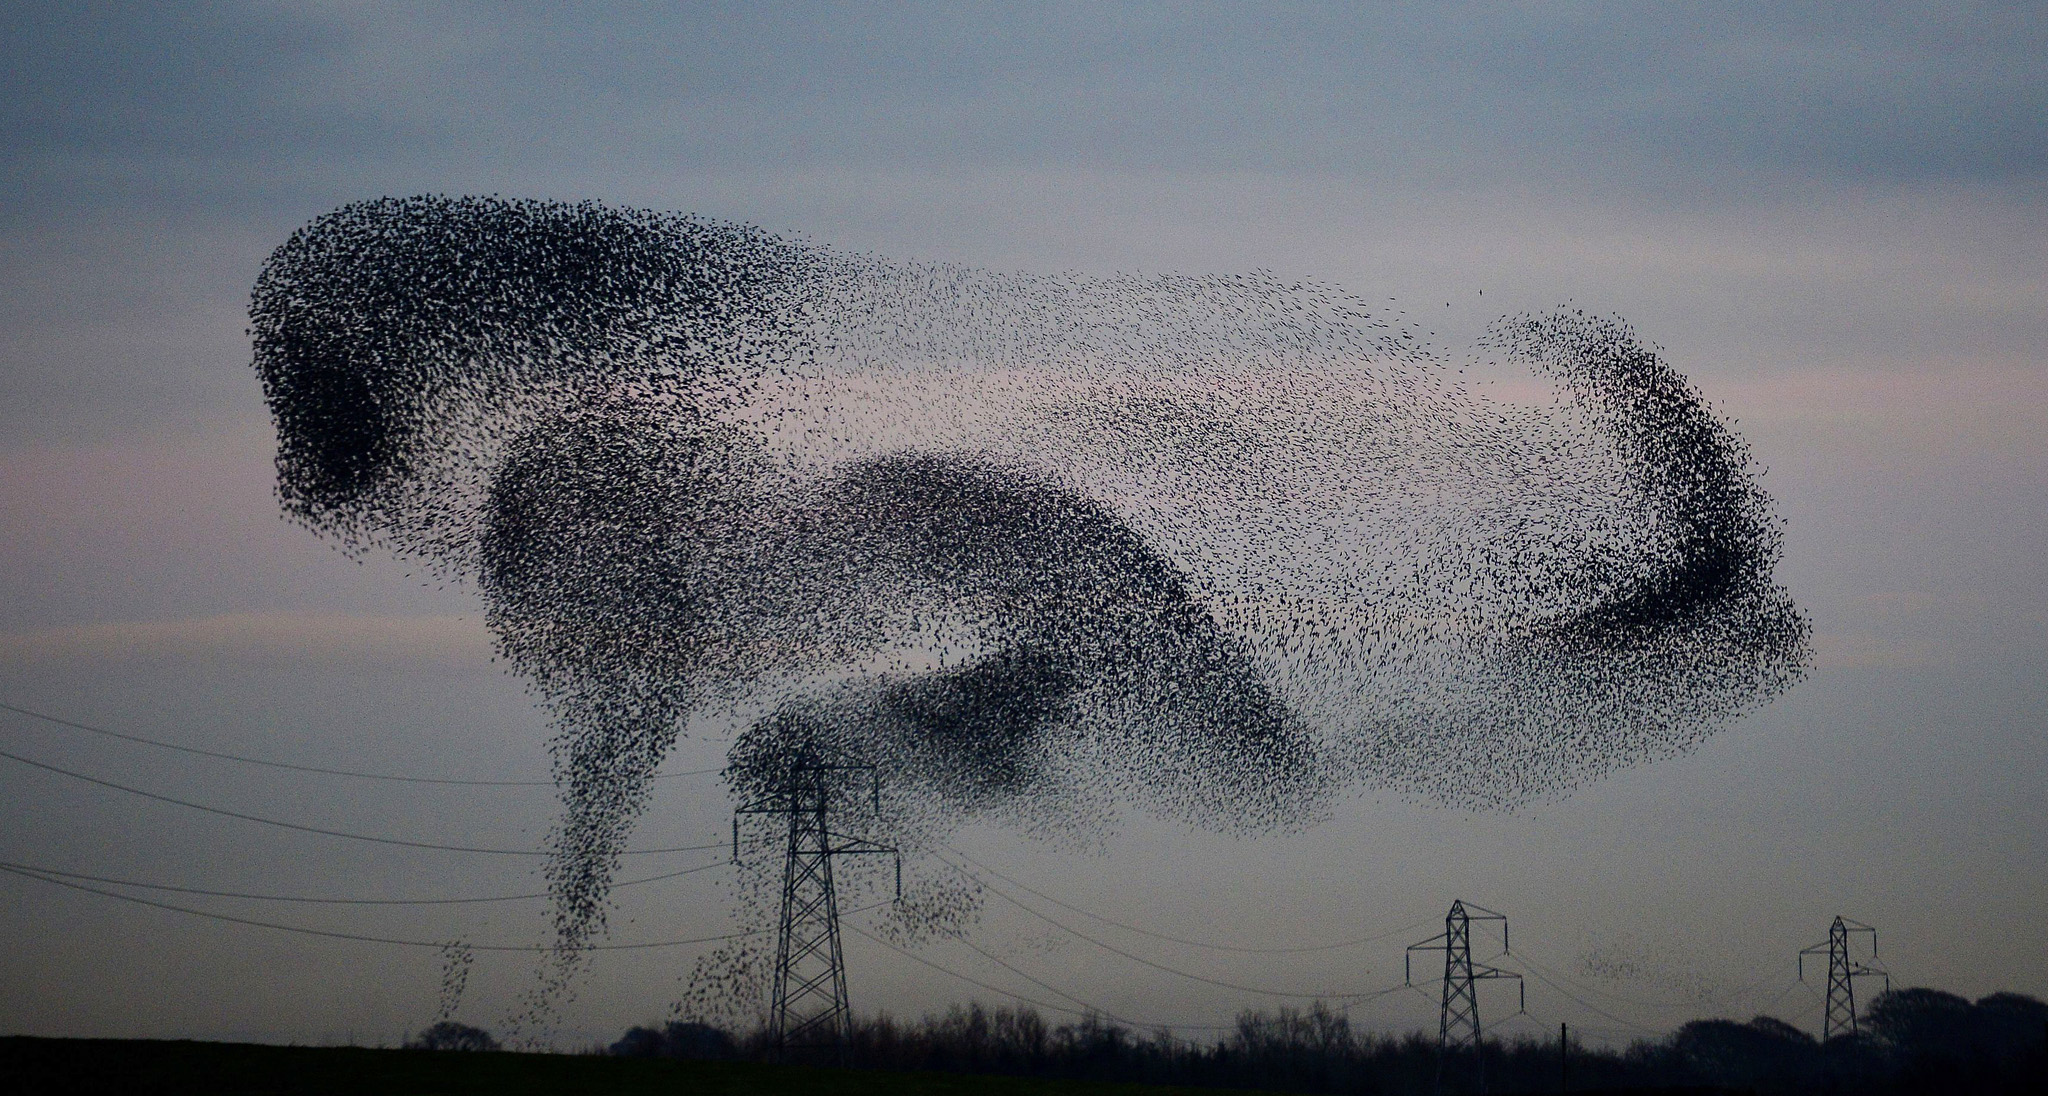
\includegraphics[width=\textwidth]{murmuration.jpg}
    \caption{A particularly startling example of a starling murmuration, captured near
        Gretna in the Scottish Borders. Photograph: Owen Humphreys/PA.}
    \label{fig:murmuration}
\end{figure}


Through captured imaginations, and over the years, collective behaviour has become a
thriving topic of multidisciplinary research, holding captive the minds of physicists,
biologists, mathematicians, and many others of the scientific persuasion. Though our
collective understanding has evolved significantly from early suggestions that collective
behaviour results from thought-transference and telepathy between individuals
\parencite{selous31}, there is still so much that remains unknown.

In many cases, the \emph{why} of collective behaviour is broadly understood. From an
evolutionary standpoint, we can reason about the benefits which collective behaviour
brings to the individuals involved. For example, it is known that aggregation can provide
an effective defence against predation \parencite{landeau86}, and that both foraging and
migration can benefit from the knowledge of the collective \parencite{simmons04}.

Despite this, much less about the \emph{how} of collective behaviour is known. The
mechanisms which lead to the formation and maintenance of aggregations remain more
elusive, and are a topic of much interest. The hope is that the study of mathematical
models of flocking, and the comparison of these models with real flocking events, will
shed light on the mechanics which underlie these phenomena. In recent years modern
computing power has made the process of simulating these models relatively pain-free,
however, a lack of quality data detailing real flocking events has made the comparison
between model and data difficult.

Previously, much work has been invested in developing the theoretical models which seek to
explain emergent behaviour by interactions at an individual level. Such models have shown
that individual interactions are sufficient to produce group-level structures
\parencite{aoki82}. Many different simulations, implementing disparate interaction rules,
are able to produce behaviour reminiscent of real flocking systems. However, these models
have largely only been verified with comparison to empirical observation at a qualitative
level, and thorough quantitative comparison between field data and theory has been
lacking. This lack of quantitative comparison between model and data can largely be
attributed to the scarcity of empirical data.

However, in recent years technological and methodological advances have made it possible
to capture the movements of large groups of animal aggregates \parencite{ballerini08}.
With this data, it is only now that we are in a position to make robust comparison
between model prediction and real-world observation.

Using recently collected data, this thesis seeks to compare newly available data of
flocking events and theoretical models. The intention is to fit multiple different models
to the same dataset. With this we will be in a position to consider which of the fitted
models best describes the observed data.

\begin{figure}[b]
    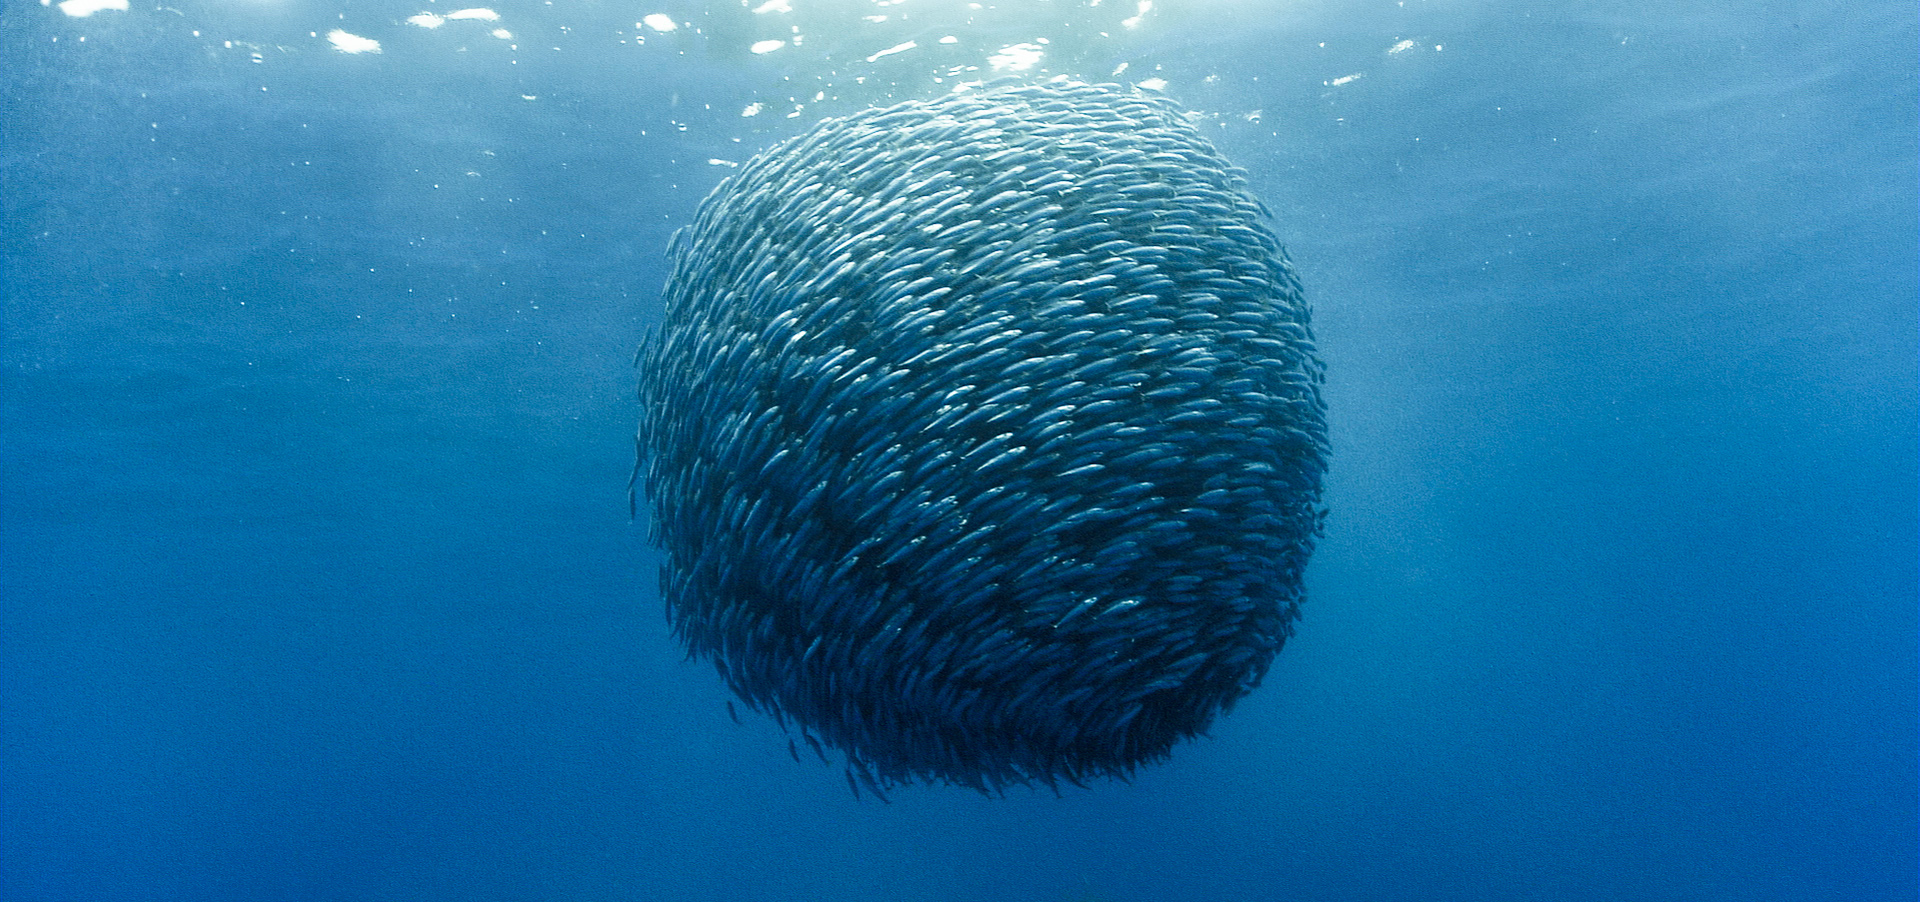
\includegraphics[width=\textwidth]{milling.jpg}
    \caption{Mackerel form a milling structure as a defence against predation.}
    \label{fig:milling}
\end{figure}

\section{Thesis overview}
\label{sec:overview_of_thesis}

We get the ball rolling in \cref{cha:lit_review} by giving the reader a
review of the literature surrounding collective behaviour. Important results and ideas of
the field are introduced and discussed. After relaying the main results from the
literature we discuss open problems and the future of research in the field.

Bayesian statistics will be introduced to the reader in \cref{cha:bayes_intro}. Important
results, techniques and algorithms from the subject will be outlined as well as any
problems that a Bayesian practitioner may encounter, and how they may address these problems.

Proceeding onwards with \cref{cha:direct_stats}, the reader will be given a short
introduction to directional statistics. Here we briefly discuss why one should take a
little extra care to avoid pitfalls when handling circular data.




  \graphicspath{{fig/lit_review/}}

\chapter{Literature review}
\label{cha:lit_review}

There exists a large body of literature relating to the phenomenon of
collective behaviour. Particularly unique to this literature is the variety of
backgrounds in which the authors are trained. Biologists, physicists, applied
mathematicians and statisticians have all made significant contributions to the
field of collective behaviour.

In this chapter we shall discuss some of the most important ideas and results
from the literature surrounding the study of collective behaviour. First, we
provide an overview and discussion of the evolutionary advantages which
collective behaviour affords individuals. After this we will discuss Eulerian
and Lagrangian models: the two main modelling paradigms used to simulate
flocking events. Finally we review previous work which focused on recording and
utilising empirical data to assess predictive performance of theoretical
models.

\section{Biological function}
\label{sec:biological_function}

Behaving as a group can bring many advantages to the individuals involved. One
classically considered benefit of aggregation is an improved defence against
predation; shoaling groups of fish have the ability to confuse predators, as
predators have difficulty selecting an individual target amongst a group (the
confusion effect) \parencite{landeau86}. In addition to this confusion effect,
groups of individuals can absorb and process more sensory information about
their environment than lone individuals are capable of, promoting the early
detection of predators \parencite{pitcher93}.

As well as providing defence against predation, behaving as a group can aid in
foraging for food as collections of individuals are able to gather more data
about their environment than solitary individuals \parencite{clark86}.
Collective motion is also understood to aid group navigation and migration,
with the suggestion that navigational accuracy increases with group size
through the ``many wrongs principle'' \parencite{simmons04}. For birds, group
navigation often brings an additional energetic advantage as individuals can
work to form aerodynamically efficient shapes \parencite{weimerskirch01}. As
well as these advantages, group living can aid in facilitating reproduction and
the rearing of young.

Despite the advantages afforded by collective behaviour, it isn't without its
dangers. For example, there is an understanding that flocking behaviours may
also have the unintended consequence of actually \emph{attracting} the
attention of predators \parencite{wittenberger85}. A more catastrophic
consequence of collective behaviour can be seen in the formation of ant mills.
Ant mills occur when a group of foraging army ants become separated from the
main column of a raiding swarm \parencite{schneirla44}. Each ant follows an
individual in front of it, causing the separated workers to run in a densely
packed circle until they eventually succumb to exhaustion
\parencite{schneirla71}. This phenomenon was first recorded in 1921, when
William Beebe observed an ant mill with a circumference of \SI{370}{\metre}
\parencite{beebe21}. It would take an individual ant \SI{2.5}{hours} to
circumnavigate a mill of this size \parencite{surowiecki05}.

As we have seen, much of the \emph{why} of collective behaviour can be
understood by considering the evolutionary advantages which group behaviour
affords the individuals involved. However, we have still yet to broach the
\emph{how} of collective behaviour.

\section{Mathematical approaches}
\label{sec:models}

There has long existed an appeal of using mathematical models as a tool to
investigate collective behaviour \parencite{aoki82, okubo86, reynolds87,
huth92, gueron93, vicsek95, couzin02}. These models of collective behaviour are
broadly partitioned into two paradigms: the Lagrangian and Eulerian approaches.
These descriptions are analogous to the models of fluid dynamics, where
Lagrangian models consider flow in terms of interactions of fluid parcels, and
Eulerian models consider the changing fluid properties at a given point in
space and time. In the analogous models of collective behaviour, Lagrangian
models simulate the movements and interactions of individuals, and Eulerian
models consider the changing properties of a group through space and time.

\subsection{Lagrangian models}
\label{ssec:lagrangian_models}

So called agent-based models (ABMs), also referred to as Lagrangian models,
have proven a useful tool in modelling collective behaviours. In these models
the behaviour of an agent is simulated at the individual level. An agent's
behaviour is determined by social interactions with neighbouring individuals.
Examples of typical interactions include the desire to move in the same
direction as neighbours (alignment, or orientation), the desire to avoid
collisions (repulsion) and a desire to remain close to neighbours (attraction).
As well as simulating social behaviours, ABMs also specify how an individual
identifies neighbours with which to interact. An agent may, for example,
identify neighbours as those; within a certain distance (metric interaction);
positioned inside a field of vision or as one of a fixed number of closest
neighbours (topological interaction).

In a pioneering paper, \textcite{aoki82} developed an ABM to simulate the
movements of fish schooling in two-dimensions. Here it was shown that
collective behaviour can arise from simple interactions at an individual level,
\emph{without} the need of a leader, and \emph{without} each individual having
information about the movement of the group as a whole. The model simulated
zonal interactions in which the area around each fish was partitioned into
zones of repulsion, alignment and attraction (correspondingly: avoid, parallel
and approach in the original publication). The partitioning of space in this
way is illustrated in \cref{fig:zone_illustration}, and has remained a popular
idea in following literature \parencite{huth92, vicsek95, couzin02, couzin05}.
This model also accounted for fish having incomplete fields of vision. The
simulation of some unobserved region was utilised in further studies. Later,
other models were also devised to simulate fish schools \parencite{okubo86,
huth92}.

\begin{figure}[tb]
  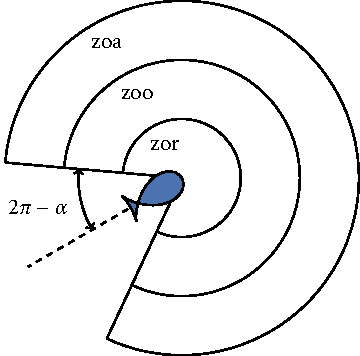
\includegraphics{zonal_tikz.pdf}
  \caption{An illustration, based on the work of \textcite{aoki82}, showing the
    area around an agent (here, a fish) partitioned into three zones; zor:
    zone of repulsion; zoo: zone of orientation (or alignment), and zoa: zone
    of attraction. The missing segment behind the individual represents a blind
    spot, of angle $2\alpha$, into which it cannot see.}
  \label{fig:zone_illustration}
\end{figure}

Following this, \textcite{reynolds87} formulated a mathematical model,
motivated by the production of computer animations, which described the
movement of birds flocking in three-dimensional space. To produce more
aesthetically pleasing animations, the software, ``Boids'', implemented
additional sophistications such as banking during turns. The focus on
developing simulations to produce visually-pleasing behaviours rendered
rigorous scientific study unbefitting. Interestingly, Tim Burton's 1992 Batman
Returns used a modified version of the Boids software to simulate animations of
bat swarms and marching penguins.

Substantially more complex than Boids was the software package Massive
(Multiple Agent Simulation System in Virtual Environment), originally developed
by Stephen Regelous for Peter Jackson's Lord of the Rings trilogy
\parencite{koeppel02}. This software was used to help generate the striking
battle sequences of the trilogy, where each individual orc, elf and other
miscellaneous creature of middle-earth was simulated according to the rules of
an agent-based model \parencite{robbins17}. In 2004, Regelous received the
Scientific and Engineering Award from the Academy of Motion Picture Arts and
Sciences for his work on Massive. Since then, Massive has been used in films
such as Inception, Harry Potter and the order of the Phoenix, James Bond's
Spectre, and HBO's hit TV series Game of Thrones (\cref{fig:got}). With this
legacy in mind, in 2018 Regelous received an Emmy award to recognise his
contribution to the entertainment industry.

\begin{figure}[tb]
  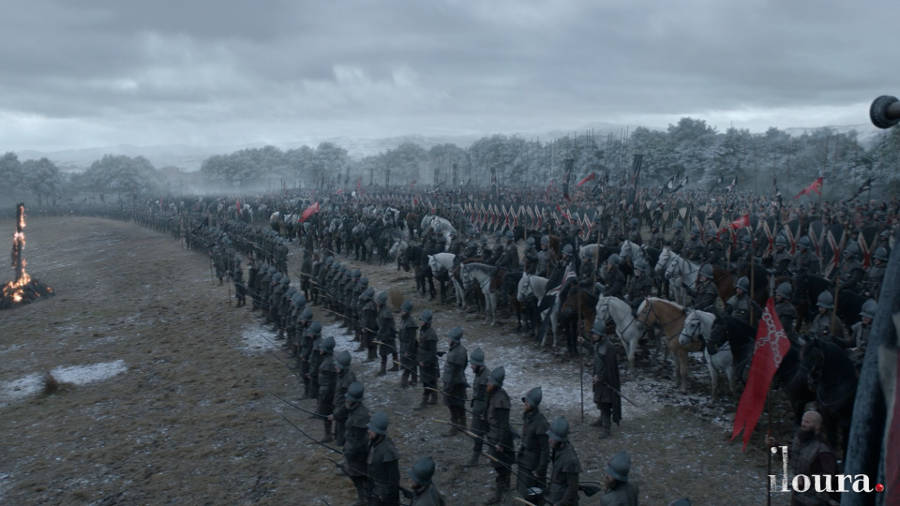
\includegraphics[width=\textwidth]{GOT.jpg}
  \caption{The animation company Iloura lent heavily on the software
    ``Massive'' to orchestrate army formations, fighting soldiers and horse
    actions for the dramatic scenes in HBO's Game of Thrones episode ``Battle
    of the Bastards''.}
  \label{fig:got}
\end{figure}

Not motivated by the lure of an Academy Award, but instead by research within
statistical physics, \textcite{vicsek95} introduced a simple two-dimensional
model in which self-propelled particles move with a fixed absolute velocity and
align with neighbours within some interaction radius. This model is commonly
referred to as the ``Vicsek Model''. Despite its simplicity this model produces
complex behaviour resembling that of a real biological system.
\textcite{vicsek95} investigated the phase transition between ordered and
disordered motion as the density of particles and noise in the system was
varied. The transition from order to disorder is an example of a spontaneously
breaking (rotational) symmetry, as the group has no preferred direction of
motion \emph{a priori}, but under simulation converges upon some arbitrary
direction of travel. Because of this, the Vicsek model stands as an apparent
violation of the Mermin-Wagner Theorem, which states that continuous symmetries
cannot be spontaneously broken by systems that are able to achieve long range
order in dimensions $d\leq 2$ \parencite{mermin66}. However, Mermin-Wagner only
applies to systems in equilibrium and the Vicsek model is out of equilibrium.

\begin{figure}[tb]
  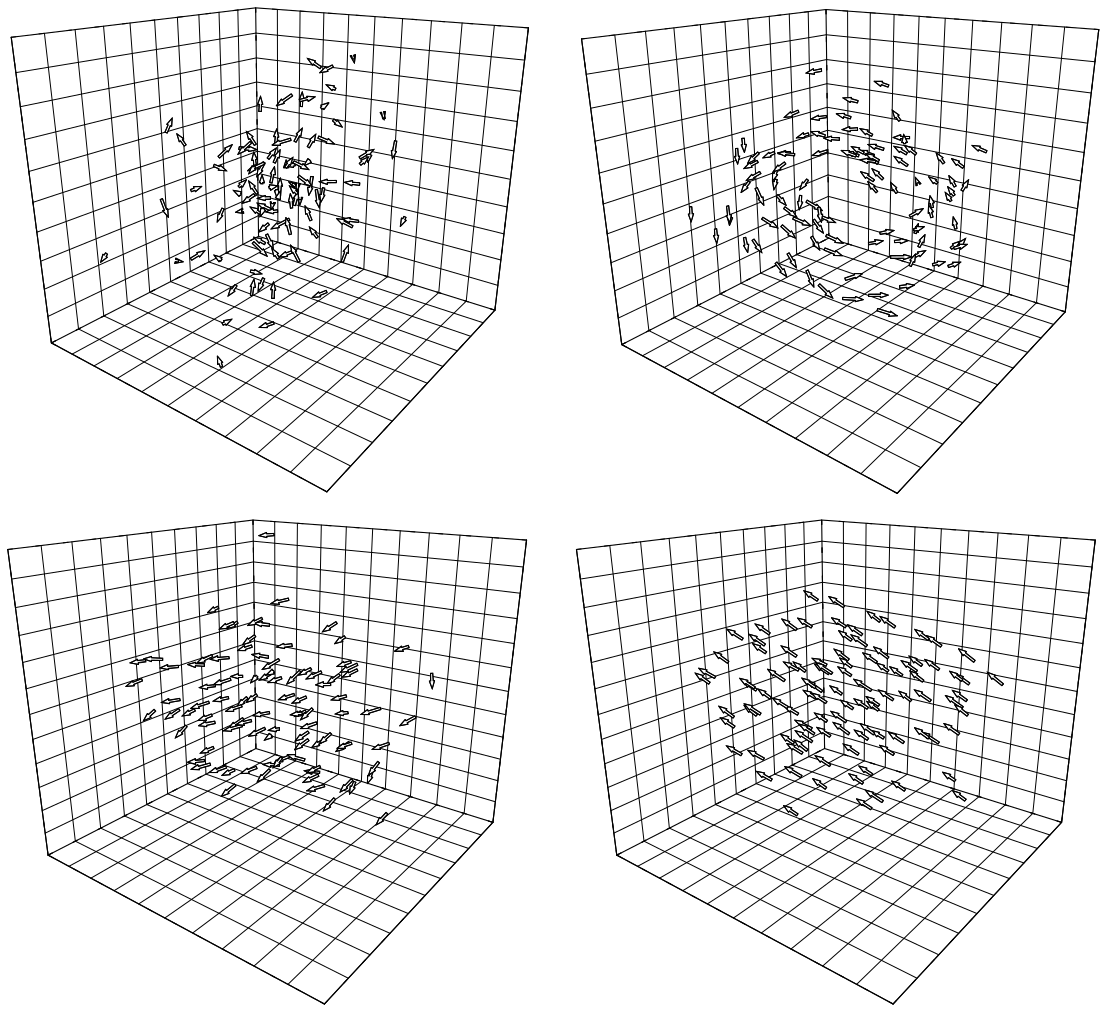
\includegraphics[width=0.75\textwidth]{couzin.png}
  \caption{Taken from \textcite{couzin02}, different steady-state
    solutions (swarm, torus, dynamically parallel and highly parallel) obtained
    by making small changes to model parameters of a three-dimensional flocking
    model.}
  \label{fig:couzin}
\end{figure}

Later models were developed to explore the movements of mammals and other
vertebrate groups. Using a three-dimensional model that follows the zonal
approach of \textcite{aoki82}, \textcite{couzin02} showed major group-level
behavioural changes as minor changes in individual interaction rules were made.
With small changes in the model parameters, groups transitioned from
disordered, swarm-like behaviour, to toroidal milling structures, to forming
dynamic and highly parallel groups, as illustrated in \cref{fig:couzin}. In
addition to this the author's simulations demonstrated evidence of the
collective memory of a group, suggesting that previous group structure
influences future behaviour as interactions change.

Further research was made by \textcite{couzin05} which investigated how leaders
influence the motion of travelling groups. A zonal
repulsion-alignment-attraction model was used as the basis for this work. Here,
though, a proportion of the flock were given information about a preferred
direction of motion, and so balanced their social interactions with the desire
to move in this direction. Individuals in the flock did not know which members
of the group, if any, had information. Simulations showed that only a small
proportion of leaders are necessary to guide groups with a high degree of
accuracy. Further results investigated how groups of individuals make
collective decisions in the face of conflicting desires.

As a method for exploring collective behaviour, Lagrangian models are very
appealing in their intuitiveness and in the ease of implementing explicit
behavioural rules. Though for many years the simulation and exploration of
these models was limited by computing power; modern computation allows for the
simulations of large groups over many time steps. With these advances in
computing, and a growing interest in the field, a significant proportion of the
literature focuses on the analysis and exploration of agent-based models.

\subsection{Eulerian models}
\label{ssec:eulerian_models}

Sometimes known as continuum models, Eulerian models are complementary to the
Lagrangian approach and work at a coarse-grained level \parencite{giardina08}.
Eulerian models are typically constructed of a set of partial differential
equations which describe how density and other group properties develop over
time. This approach to modelling is often used to investigate the long-time
spatial and density properties of groups.

One such Eulerian approach by \textcite{gueron93} modelled the movements of
large groups of wildebeest. Their model predictions were compared with aerial
observations of wildebeest migrating through the Serengeti
(\cref{fig:wildebeest}). The large-scale front patterns seen in the aerial
photography were reproduced by their model.

\begin{figure}[tb]
  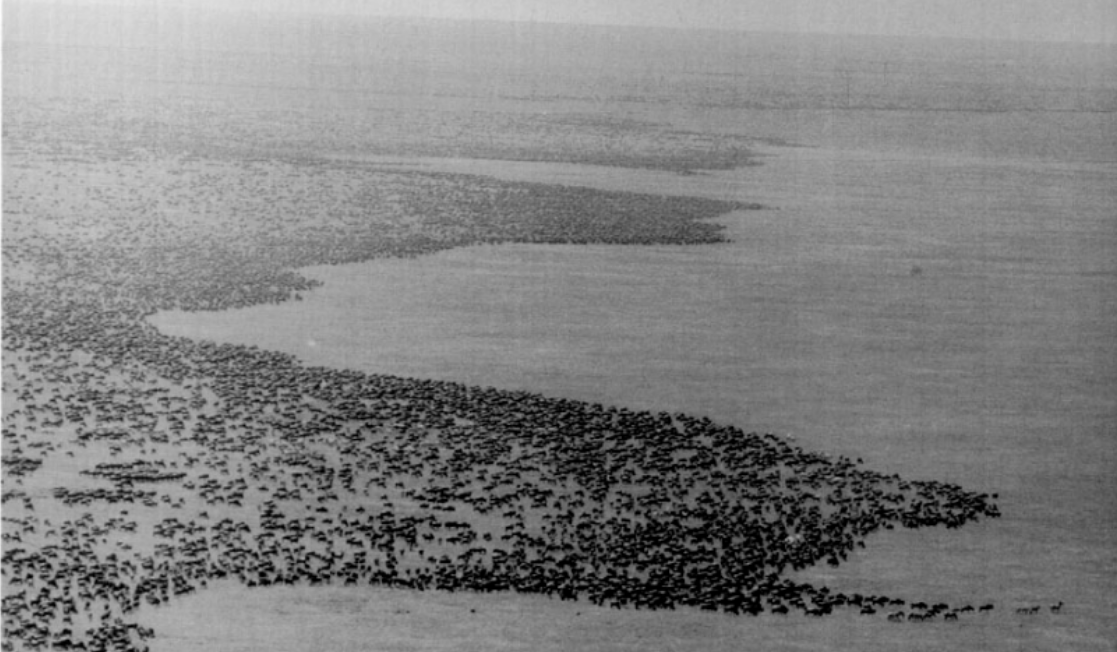
\includegraphics[width=\textwidth]{wildebeest.png}
  \caption{Aerial photography of migrating wildebeest showing large-scale
    front patterns, as presented in the work of \textcite{gueron93}.}
  \label{fig:wildebeest}
\end{figure}

Later, \textcite{toner98} introduced a quantitative continuum theory of
flocking. There are similarities between the hydrodynamic equations introduced
by the authors and the Navier-Stokes equation for simple incompressible fluids.
This model is capable of predicting the existence of an ordered phase of
motion, as is often observed in the field, and propagating density waves.
Detailed analysis of the model is made using techniques (e.g. dynamical
renormalisation group) from nonequilibrium condensed matter physics and can be
used to make quantitative predictions of the properties of the long-distance,
long-time behaviour of the ordered state. Eulerian models have also been used
to analyse vortex and stationary clump solutions \parencite{topaz04,topaz06}.

However, the Eulerian approach is limited. Most analyses are restricted to a
single dimension and the approach has not proven appropriate for modelling
groups of low densities \parencite{giardina08}. Additionally, these models
require more involved computer implementation than their Lagrangian
counterparts necessitate. With this in mind, and with the advantages of the
Lagrangian approach, in this thesis we will concentrate entirely on modelling
in the Lagrangian framework.

\section{Empirical studies}
\label{sec:empirical_studies}

Models of collective motion rely on aprioristic assumptions about the
properties and behaviours of individuals. It is understood that the emergence
of a biologically realistic pattern from model simulation \emph{is not}
sufficient evidence of model correctness. That is, the emergence of a desired
pattern is not sufficient evidence that a model is correctly capturing the
interactions between individuals. This observation is further compounded by the
understanding that models implementing different local interactions can produce
similar looking behaviour at the group level; see, for instance, the similar
behaviours (swarms, undirected mills and moving aligned groups) exhibited by
the zonal repulsion-alignment-attraction model of \textcite{couzin02} and the
attraction-blind-angle model of \textcite{strombom11}.

As such, real data describing the dynamics of animal aggregations is
\emph{essential} to assess the validity and efficacy of theoretical models and
the assumptions they make. With such data it becomes possible to compare and
rank the predictive performance of competing models.

Thorough comparison between model and data has proven difficult largely
because of the scarcity of appropriate data. The collection of suitable data
can be a complicated and convoluted process. Taking observations in the field
is technically demanding, requiring the precise calibration of sensitive
measuring equipment, not to mention the additional difficulty imposed by the
typically three-dimensional nature of animal aggregations. Collecting data in a
laboratory setting seems an obvious workaround, however this imposes
restrictions on the types of behaviour which can be captured; a laboratory may
be an appropriate environment to capture the movements of fish in a tank, but
it certainly isn't appropriate to capture the behaviour of flocking birds.
Despite the difficulties associated with collecting data, significant effort
has been made to track the movements and dynamics of groups of individuals.

\begin{figure}[tb]
  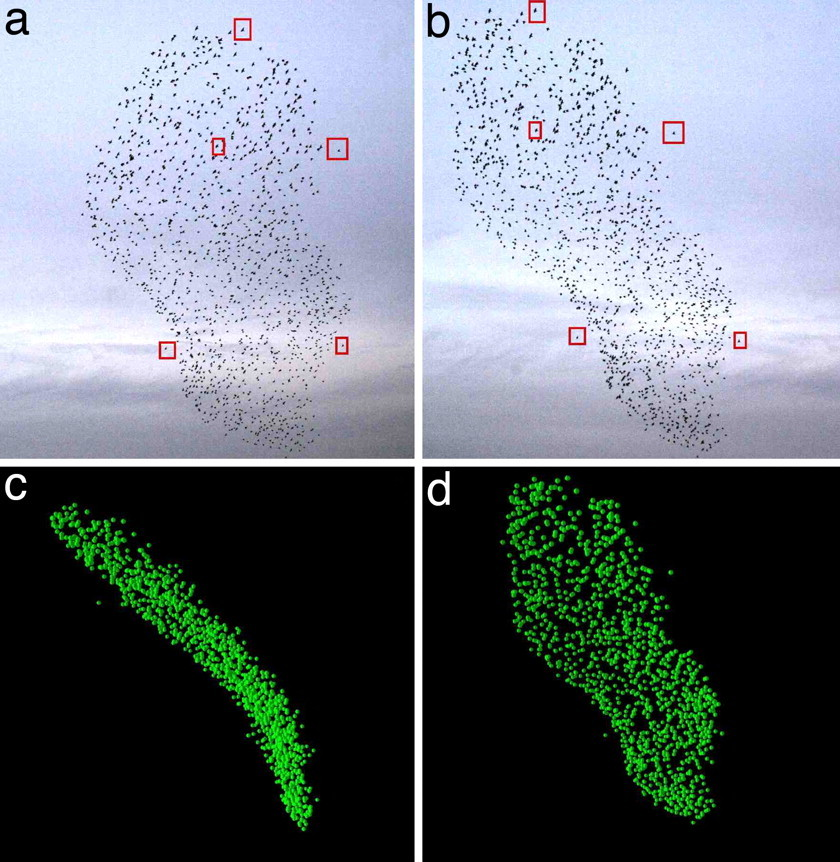
\includegraphics[width=0.75\textwidth]{ballerini_starlings.jpg}
  \caption{A flock of 1246 starlings reconstructed in three-dimensions.
    Photographs taken at the same instant but \SI{25}{\meter} apart (a--b) are used
    to reconstruct their three-dimensional positions (c--d). To perform
    reconstruction \textcite{ballerini08} needed to match each bird in (a)
    to its corresponding position in (b). The red squares show five matched
    pairs of birds.}
  \label{fig:ballerini}
\end{figure}

Initial work was limited to tracking small numbers of individuals in groups. In
these studies individuals were not linked between frames and hence the
collected data had no dynamic component. The first breakthrough came from
\textcite{cullen65} who used stereo photography to record the positions of fish
in three-dimensions.

Fish are an appealing subject to study as experiments are easily conducted in a
laboratory setting. Furthermore, the movements of fish can effectively be
restricted to two-dimensions by conducting the experiments in shallow water.
With these considerations, further research also concentrated on fish
\parencite{partridge80,van_long85}. Having collected empirical data, these
studies investigate properties such as the distance of individuals to their
nearest neighbour, or the direction from an individual toward their nearest
neighbour. Empirical studies were also made of small groups of flocking birds,
with similar statistics and properties realised \parencite{major78,budgey98}.

More recently, a breakthrough study by \textcite{ballerini08} reconstructed the
three-dimensional positions of flocks of starlings consisting of up to 2600
individuals (\cref{fig:ballerini}). To collect this data the authors
used a combination of stereometric and computer vision techniques. Having
extracted the data, the authors began by constructing angular
density plots of nearest neighbours. These plots revealed a strong anisotropy
in the flock, with a lack of nearest neighbours positioned along the direction
of motion. Having investigated how this anisotropy decays as a function of
nearest neighbour, the authors concluded that interactions are not dependent on
metric distance (interactions with agents within a fixed distance), as most
models in the literature assume, but on a topological distance (interaction
with a fixed number of closest agents, irrespective of distance). This analysis
suggested that on average a starling interacts with between six and seven of
its closest neighbours.

\begin{figure}[tb]
  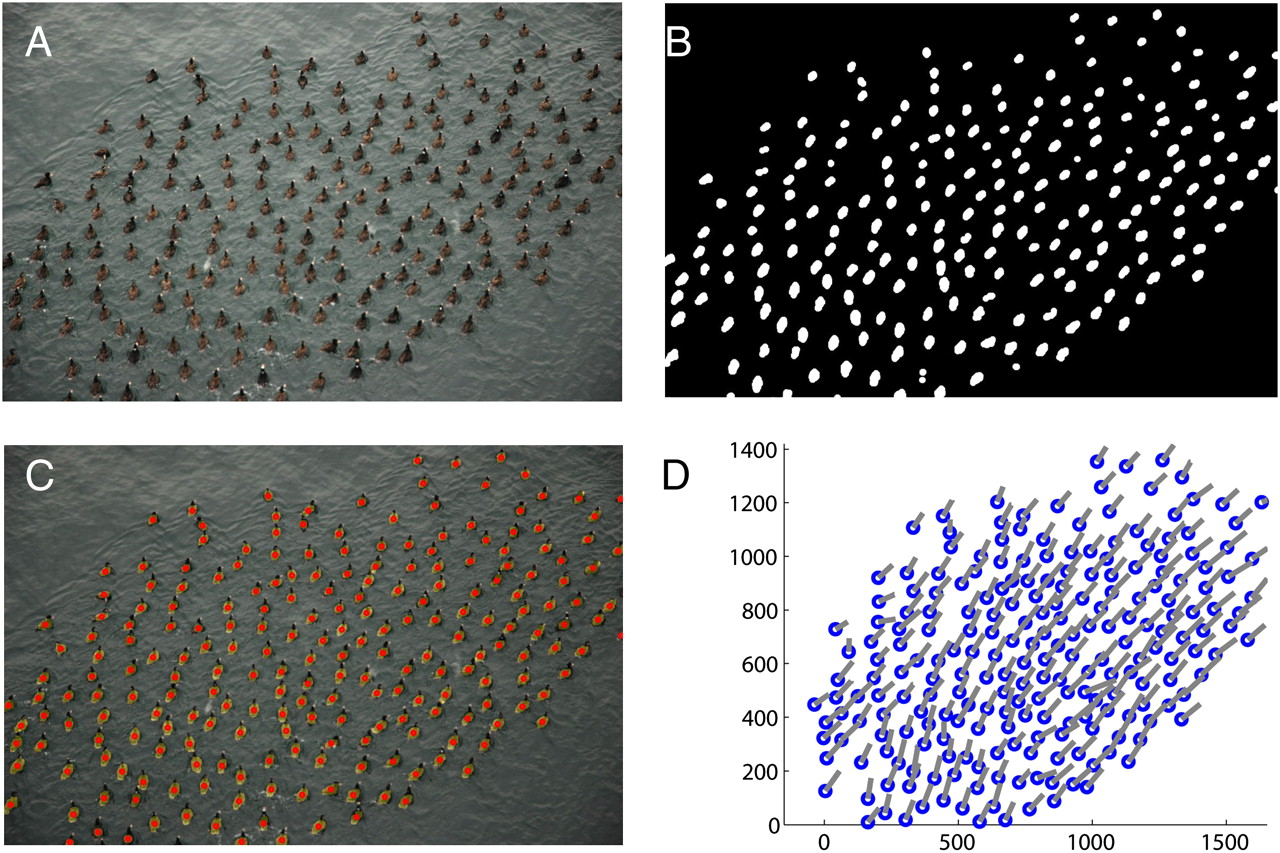
\includegraphics[width=\textwidth]{lukeman_data.jpg}
  \caption{An image of field data and visualisations of the transformations
    used to extract positions of individuals in a flock of foraging birds 
    \parencite{lukeman10}.}
  \label{fig:lukeman_extraction}
\end{figure}

A significant contribution to the field was made by \textcite{lukeman10}, who
collected and analysed data of large flocks of ducks interacting on the surface
of a lake. Crucially, this dataset tracked individuals \emph{between} frames
and therefore allowed the reconstruction of a bird's trajectory through space
and time. This data showed an increase by a factor of ten the number of
individuals which could be reliably tracked though time \parencite{lukeman09}.
Plots of nearest neighbour densities were constructed from the extracted
dataset. It was observed from these plots that the highest density of
neighbours occurs at some preferred distance in front of and behind the focal
bird. Further analysis fitted varying zonal models to the data. Model
parameters were fitted which could best reproduce angular and radial neighbour
distributions. It was concluded that a zonal repulsion-alignment-attraction
model with an additional frontal interaction was best able to reproduce the
desired neighbour distributions.

Following this, \cite{katz11} investigated two and three fish shoals of golden
shiners. Data was recorded by placing fish in shallow tanks of water and using
custom tracking software to convert video footage into data describing the
centre of mass of individual fish through time. Working in a classical
mechanics framework the authors considered the effective forces acting on a
focal fish as a function of position and velocity. The authors found that the
dominant interaction between fish was the regulation of their speed. No
evidence was found of an explicit alignment interaction between individuals;
instead, alignment occurred as a product of attraction and repulsion between
individuals. Pairwise interactions were seen to predict the spatial
distributions of neighbours, and this observation was validated for shoals of
10 and 30 individuals.

With many different models capable of producing realistic-looking flocks,
researchers have sought to make quantitative comparison between the
model-performance using techniques from the model-selection literature.
\textcite{mann13} fit a number of models---including a topological model, a
non-local model (in which all agents interact), and a variety of different
spatial models---to data describing the collective motion of glass prawns. In
computing the marginal log-likelihood of candidate models the authors were able
to conclude that a spatial model with a persistent ``memory'' effect provided
the best fit to data.

The marginal log-likelihood provides an appealing measure with which to compare
model fits: penalising models for complexity, and favouring simpler models.
Following the methodology outlined by \textcite{mann13},
\textcite{strandburg13} used the marginal log-likelihood to compare models with
metric, topological, Voronoi and visual interaction rules. Although the
marginal-likelihood is often used to compare model performance, under certain
situations the marginal-likelihood is also understood to be highly sensitive to
prior dispersion, even when the posterior is robust against prior dispersion
\parencite{fong20}. As such, information-criterion approximations to the
marginal-likelihood represent popular alternatives.

Analysis of empirical data has so far focused on epiphenomena such as nearest
neighbour distances or angular neighbour densities. Research has then focused
on fitting models which are best able to replicate these properties, rather
than movements of individuals themselves. With technological and methodological
advances we expect that more and more empirical data will become available in
the future.

\section{Numerical studies}
\label{sec:numerical_studies}

\textcite{mann11} acknowledged that an important aspect of model fitting is
knowing the associated uncertainty of inferred parameters. The author discussed
the importance of quantifying uncertainty in parameter inference on collective
behaviour models, as the associated empirical datasets often have high levels
of noise. With the importance of capturing uncertainty in mind, Mann
demonstrated a fully Bayesian approach to parameter inference on data simulated
from a collective behaviour model. Here, in contrast to the more numerous
empirical studies, parameters were inferred on their ability to explain the
\emph{movements} of agents, as opposed to the ability to reproduce epiphenomena
such as nearest neighbour densities or angular neighbour distributions.

The agents in Mann's model moved under a weighted sum of alignment and
attraction. After ten time steps the simulated data transitioned from
disordered motion to a steady state rotating mill. The author then compared the
ability to infer the weighting parameter, interaction radius and other
properties of the agents in two situations: before and after the achievement of
a steady state. It was discovered that the interaction radius could not be
reliably inferred when the agents had formed the rotating mill structure,
although it could be inferred in the disordered motion before steady state.
This result can be understood by considering that stable groups present a
limited number of particle configurations, and are therefore less informative
than out of equilibrium groups.

Although not utilised frequently in the literature, such simulation studies
represent a useful aid in developing the statistical machinery to fit models of
collective behaviour to real data.

\section*{Conclusions}

Although our understanding of collective behaviour has developed considerably
from early speculations of telepathy, there still remain \emph{many} unknowns.
We saw that the notion of biological fitness goes a long way to explaining the
\emph{why} of collective behaviour. However, we also reflected on how much is
unknown about the \emph{how} of collective behaviour.

Much of the literature was seen to have utilised mathematical models in an
attempt to understand the mechanics underlying the formation and maintenance of
flocks. Two popular modelling paradigms were introduced: Eulerian, and
Lagrangian. Considering the strengths and weaknesses of these approaches, we
concluded that the Lagrangian framework represents a more intuitive and
appealing paradigm for our study of collective behaviour.

Having considered a number of Lagrangian models, we saw that a variety of
different models were able to produce visually similar flocking events. We
argued that comparison between model and data is essential to assess the
performance and realism of theoretical models. A review of the literature
taking measure of real flocking events was detailed. Previous work has been
limited by the availability of data of flocking events. When data of real
events \emph{has} been utilised, the focus has been on fitting models to best
reproduce properties such as nearest-neighbour densities. We argue that the
fitting process should instead centre on explaining the \emph{movements} of the
flock, rather than some epiphenomena of their movements.

In this thesis we seek to address the shortcomings of previous work. In
particular, we seek to fit theoretical models of collective behaviour to
observations of real events. In contrast with previous work, this fitting
process will seek to explain the \emph{movements} of flocks, rather than some
statistical properties of the flocks. Parameter uncertainty will be quantified
in all subsequent analyses. In addition to this, multiple competing models will
be fit to the same observations, allowing us to perform a quantitative
comparison of predictive performance, and assess aprioristic modelling
assumptions.

  \graphicspath{{fig/bayes_intro/}}

\chapter{Bayesian statistics}
\label{cha:bayes_intro}
In this thesis we utilise techniques from Bayesian inference to fit theoretical models of collective behaviour to real data. Bayesian inference allows the practitioner to capture uncertainty about fitted model parameters. In addition to this the Bayesian framework permits flexible model structures and potential inclusion of expert information via the prior distribution. With this we seek to fit empirical data to a generalisation of a popular model from the literature.

In this chapter we shall introduce and give overviews of some important concepts of Bayesian inference, outline schemes which can be used to infer model parameters, and discuss some of the problems which may arise and how we might address them.

\section{Bayesian inference}
\label{sec:bayesian_inference}
Using Bayesian inference we wish to quantify beliefs and uncertainties about parameters $\bm{\theta} = (\theta_1, \theta_2,\dots,\theta_p)^T$, using data $\bm{x}$ which we observe. Given this observed data, the likelihood function for the parameters is defined
\[
    L(\bm{\theta}\given\bm{x}) = f(\bm{x} \given \bm{\theta}).
\]
The likelihood quantifies the probability distribution of the data in terms of the parameters. We may then specify our prior knowledge about the parameters $\bm{\theta}$ through the prior distribution $\pi(\bm{\theta})$. Bayes Theorem can then be used to incorporate both the likelihood function and our prior beliefs, to form the posterior distribution
\begin{equation}
\label{eq:bayes_theorem}
    \pi(\bm{\theta}\given\bm{x}) = \frac{\pi({\bm{\theta}})L(\bm{\theta}\given\bm{x})}{\int_{\bm{\theta}} \pi(\bm{\theta})L(\bm{\theta}\given\bm{x}) \, \textup{d}\bm{\theta}}.
\end{equation}
Because the integral in the denominator is not a function of $\bm{\theta}$, we may consider it a constant of proportionality and express our posterior beliefs as proportional to the product of the likelihood and prior, that is
\begin{align*}
    \pi(\bm{\theta}\given\bm{x}) &\propto \pi(\bm{\theta}) \times L(\bm{\theta}\given\bm{x})\\
    \text{posterior} &\propto \text{prior} \times \text{likelihood}
\end{align*}

\section{Markov chain Monte Carlo (MCMC)}
\label{sec:mcmc}
For the most part, the normalising constant (given in the denominator of \cref{eq:bayes_theorem}) will have multiple dimensions, not produce a density function of standard form, and be difficult to evaluate in all but the most trivial cases. Markov chain Monte Carlo algorithms provide methods to sample from the targeted density $\pi(\bm{\theta} \given \bm{x})$, whilst avoiding evaluating the troublesome normalising constant.

\subsection{Gibbs sampling}
\label{ssec:gibbs_sampling}
One may use the full conditional distributions of parameters to sample from a multivariate density. Doing so is to implement the Gibbs algorithm. So, instead of sampling from the full posterior, we sample from the conditional posteriors of the parameters one at a time. The Gibbs algorithm is useful when the conditional densities can be expressed in standard form and are easy to sample form.

Say we wish to target the density $\pi(\bm{\theta})$ where $\bm{\theta} = (\theta_1, \theta_2, \dots, \theta_p)^T$, where the full conditional densities are $\pi(\theta_i \given \theta_1, \theta_2, \dots, \theta_{i-1}, \theta_{i+1}, \dots, \theta_p)$, for $i=1,\dots,p$, then we may use the Gibbs sampler, as described in \cref{alg:gibbs}.

\begin{algorithm}[htbp]
	\begin{enumerate}
	    \setcounter{enumi}{-1}
	    \item Initialise chain with $\bm{\theta}^{0}$. Set $j=1$.
	    \item Generate $\bm{\theta}^{j}$ from $\bm{\theta}^{j-1}$ by simulating from:
	    \begin{align*}
	            {\theta_1}^{j} &\sim \pi({\theta_1}^{j} \given {\theta_2}^{j-1},\dots,{\theta_p}^{j-1},\bm{x})\\
	            {\theta_2}^{j} &\sim \pi({\theta_2}^{j} \given {\theta_1}^{j}, {\theta_3}^{j-1}, \dots, {\theta_p}^{j-1},\bm{x})\\
	            &\hspace{0.25cm}\vdots \\
	            {\theta_p}^{j} &\sim \pi({\theta_n}^{j} \given {\theta_1}^{j}, \dots, {\theta_{p-1}}^{j-1},\bm{x})
	    \end{align*}
	    \item Increment $j$ to $j+1$. Repeat from step $1$.
	\end{enumerate}
	\caption{Gibbs Algorithm targeting the density $\pi(\bm{\theta} \given \bm{x})$.}
	\label{alg:gibbs}
\end{algorithm}

\subsection{Metropolis-Hastings}
\label{ssec:metropolis_hastings}
The Metropolis-Hastings algorithm is another MCMC scheme. The algorithm was introduced by \cite{metropolis53}, and this work was later generalised by \cite{hastings70}. The algorithm works by constructing a Markov chain which has stationary distribution equivalent to the distribution of interest.

% Add thin space after \min ???
\begin{algorithm}[htbp]
	\begin{enumerate}
	    \setcounter{enumi}{-1}
	    \item Initialise chain with $\bm{\theta}^{0}$. Set $j=1$.
	    \item Propose ${\bm{\theta}}^\star$ by sampling from $q(\cdot \given {\bm{\theta}}^{j-1})$, where $q$ is some proposal distribution
	    \item Construct the acceptance probability $\alpha({\bm{\theta}}^\star \given {\bm{\theta}^{j-1}})$ as
	    \begin{equation*}
			\alpha({\bm{\theta}}^\star \given \bm{\theta}) = \min\bigg\{ 1, \frac{\pi({\bm{\theta}}^\star)}{\pi({\bm{\theta}}^{j-1})} \frac{L(\bm{\theta}^\star \given \bm{x})}{L({\bm{\theta}}^{j-1} \given \bm{x})} \frac{q({\bm{\theta}}^{j-1} \given {\bm{\theta}}^\star)}{q({\bm{\theta}}^\star \given {\bm{\theta}}^{j-1})} \bigg\}.
	    \end{equation*}
	    \item With probability $\alpha({\bm{\theta}}^\star \given {\bm{\theta}^{j-1}})$ set ${\bm{\theta}}^j = {\bm{\theta}}^\star$, otherwise set ${\bm{\theta}}^j = {\bm{\theta}}^{j-1}$.
	    \item Increment $j$ to $j+1$. Repeat from step $1$.
	\end{enumerate}
	\caption{The Metropolis-Hastings used to target the posterior distribution $\pi(\bm{\theta} \given \bm{x})$.}
	\label{alg:metropolis_hastings}
\end{algorithm}

The algorithm begins by initialising the chain with parameters $\bm{\theta}^{0}$. Next, the algorithm proposes new values ${\bm{\theta}}^\star$ from a proposal distribution, $q(\bm{\theta}^\star \given {\bm{\theta}}^{j-1})$, which is chosen to have the same support as the target distribution. After this, the proposed values ${\bm{\theta}}^\star$ are either accepted or rejected, depending on the evaluation of the acceptance probability $\alpha({\bm{\theta}}^\star \given {\bm{\theta}^{j-1}})$. Because the acceptance probability depends on a ratio of $\pi(\cdot \given \bm{x})$, the normalising constants cancel and therefore the target distribution only has to be known to a constant of proportionality. Metropolis-Hastings is described more formally in \cref{alg:metropolis_hastings}.

\subsubsection{Choosing a Proposal Distribution}
\label{ssec:proposal_distribution}
The practitioner must choose a suitable proposal distribution $q(\bm{\theta}^\star \given \bm{\theta})$. Ideally the choice of proposal distribution will give rapid convergence to $\pi(\bm{\theta} \given \bm{x})$ and efficiently explore the support of $\pi(\bm{\theta} \given \bm{x})$.

A special case of Metropolis-Hastings arises when the proposal distribution is symmetric, that is
\begin{equation*}
	q(\bm{\theta}^\star \given \bm{\theta}) = q(\bm{\theta} \given \bm{\theta}^\star).
\end{equation*}
In this case we observe cancellation in the acceptance ratio, as it simplifies to become 
\begin{equation*}
	\alpha({\bm{\theta}}^\star \given \bm{\theta}) = \text{min}\bigg\{ 1, \frac{\pi({\bm{\theta}}^\star)}{\pi({\bm{\theta}}^{j-1})} \frac{L(\bm{\theta}^\star \given \bm{x})}{L({\bm{\theta}}^{j-1} \given \bm{x})} \bigg\}.
\end{equation*}

Another special case of Metropolis-Hastings is the random walk sampler. In this case proposals are realised as
\begin{equation*}
	\bm{\theta}^\star = \bm{\theta}^{j-1} + \bm{\omega}^{j-1},
\end{equation*}
where the $\bm{\omega}$ are drawn from
\begin{equation*}
	\bm{\omega}^{j-1} \sim \mathcal{N}_p(\bm{0}, \Sigma),
\end{equation*}
and $\mathcal{N}_p$ denotes a $p$--dimensional multivariate normal distribution. The parameter $\Sigma$ is called the tuning parameter and controls how the chain moves around the parameter space. Mixing describes how efficiently the chain moves around the sample space and how long it takes for the chain to converge to the target distribution.

Crucially then, the parameter $\Sigma$ controls the mixing of the chain. So, naturally, we wish to select some optimum $\Sigma$ to try and improve mixing. If the target distribution is Gaussian, it has been shown that 0.234 is an optimum acceptance probability \parencite{roberts01}. In an attempt to tune $\Sigma$ to obtain the optimum acceptance probability, a common technique is to use 
\begin{equation*}
	\Sigma = \frac{2.38^2}{p} \widehat{\text{Var}}(\bm{\theta} \given \bm{x}).
\end{equation*}

\subsubsection{Blocking Parameters}
\label{ssec:blocking}
In the schemes considered so far the proposal, acceptance and rejection of the entire parameter space $\bm{\theta}$ happened simultaneously. This approach becomes inefficient for high-dimensional problems. Consider that as the dimension of the problem increases, the chances of proposing a value $\theta_i^\star$ in the tails of the posterior distribution increases. Increasing the chance of proposing a component $\theta_i$ out in the tails of the distribution in turn decreases the acceptance rate of the chain and leads to slower convergence.

To overcome this problem the parameter space $\bm{\theta}$ can be split into blocks of parameters $\bm{\theta}_1, \ldots, \bm{\theta}_d$ which are proposed and accepted or rejected separately. There are no theoretical results which determine how best to block the parameter space, though typically blocks are chosen to contain related parameters.

Blocking doesn't reduce the risk of a parameter being proposed in the tails of the distribution, however when such a proposal does occur only a subset of all the chains are affected. In this way blocking can alleviate the lower acceptance rates that are associated with high dimensionality.

There is, however, an additional computational cost that comes with blocking parameters. Consider that if the parameter space $\bm{\theta}$ is partitioned into $d$ blocks, then for each iteration of the scheme the acceptance ratio, and therefore the likelihood, proposal density and prior distribution must be evaluated $d$ times. In application the practitioner will likely seek some compromise between acceptance rate and computation time.

\subsection{Convergence Diagnostics}
\label{ssec:convergence_diagnostics}
Though there are theoretical methods to assess the convergence of chains, it is an attractive idea to analyse the output of our schemes in an attempt to assess whether the chains have converged. One of the simplest informal methods to assess convergence is to inspect the trace plots of the scheme and check for any irregularities. It is also good to use autocorrelation plots to assess autocorrelation between samples at different lags.

One way to lower autocorrelation between samples is to thin the output. When thinning, every $k$-th sample from a chain is kept and the remaining samples are discarded. Another common technique is to allow for a burn-in period. The purpose of a burn-in period is to discard any samples from before the chain has converged.

  %\appendix

  %\begin{chapter}{\label{app:appendix_label}My appendix title}

\end{chapter}
                    % An appendix.

  % Uncomment the line below if you want your Bibliography to appear in the
  % table of contents.
  %\addcontentsline{toc}{chapter}{Bibliography}
  \bibliography{references}             % References.
  \bibliographystyle{inputs/jfm}

\end{document}
